\documentclass[tikz]{standalone}
\usepackage{bm}
\begin{document}
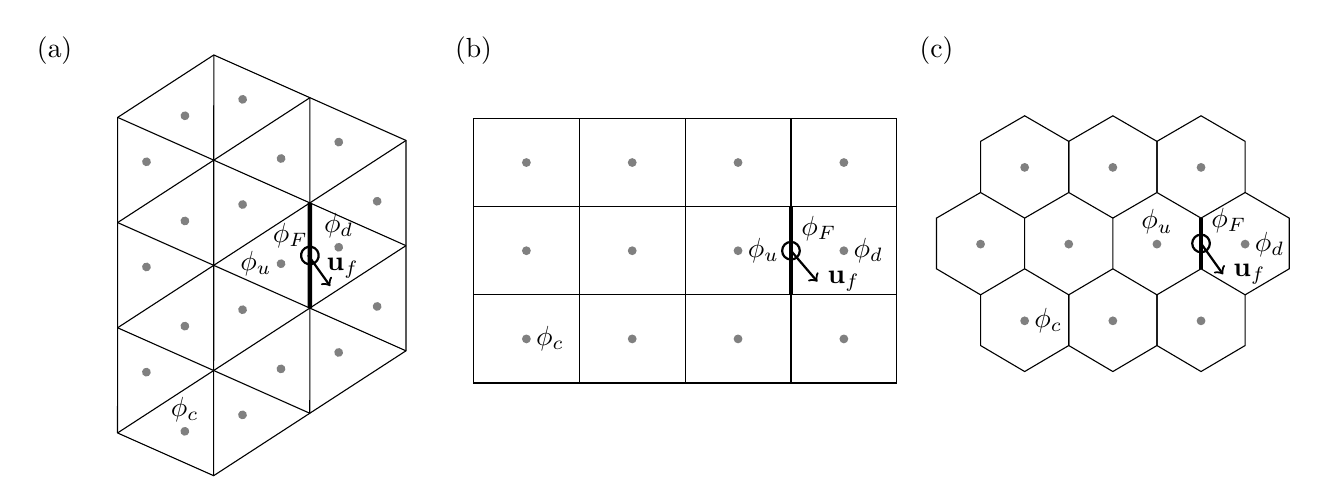
\begin{tikzpicture}[
  scale=0.56,
  cpnt/.style={fill=gray},
]

\node [above] at (0.5,7) {(a)};
\draw [thick, ->] (6.25,2.9) -- (6.75,2.2);
\node [right] at (6.45,2.6) {$\mathbf{u}_f$};

\begin{scope}[rotate=33,shift={(1,-4)}]
	\draw (0,2) -- (1.3,0) -- (6.5,0) -- (9.1,4) -- (6.5,8) -- (3.9,8) -- (0,2);

	\draw (0,2) -- (7.8,2);
	\draw (1.3,4) -- (9.1,4);
	\draw (2.6,6) -- (7.8,6);

	\draw (1.3,0) -- (6.5,8);
	\draw (3.9,0) -- (7.8,6);
	\draw (1.3,4) -- (3.9,0);
	\draw (2.6,6) -- (6.5,0);
	\draw (3.9,8) -- (7.8,2);

	\path [cpnt] (1.3,1.2) circle [radius=0.1] node [above] {$\phi_c$};
	\path [cpnt] (2.6,0.8) circle [radius=0.1];
	\path [cpnt] (3.9,1.2) circle [radius=0.1];
	\path [cpnt] (5.2,0.8) circle [radius=0.1];
	\path [cpnt] (6.5,1.2) circle [radius=0.1];

	\path [cpnt] (1.3,2.8) circle [radius=0.1];
	\path [cpnt] (2.6,3.2) circle [radius=0.1];
	\path [cpnt] (3.9,2.8) circle [radius=0.1];
	\path [cpnt] (5.2,3.2) circle [radius=0.1] node [left] {$\phi_u$};
	\path [cpnt] (6.5,2.8) circle [radius=0.1] node [above] {$\phi_d$};
	\path [cpnt] (7.8,3.2) circle [radius=0.1];

	\path [cpnt] (2.6,4.8) circle [radius=0.1];
	\path [cpnt] (3.9,5.2) circle [radius=0.1];
	\path [cpnt] (5.2,4.8) circle [radius=0.1];
	\path [cpnt] (6.5,5.2) circle [radius=0.1];
	\path [cpnt] (7.8,4.8) circle [radius=0.1];

	\path [cpnt] (3.9,6.8) circle [radius=0.1];
	\path [cpnt] (5.2,7.2) circle [radius=0.1];
	\path [cpnt] (6.5,6.8) circle [radius=0.1];

	\draw [ultra thick] (5.2,2) -- (6.5,4);
	\draw [thick] (5.85,3) circle [radius=0.2];
	\node at (5.45,3.2) [above] {$\phi_F$};
\end{scope}

\begin{scope}[shift={(10,0)}]
	\node [above] at (0,7) {(b)};
	\draw (0,0) rectangle (9.6,6);
	\draw (0,2) -- (9.6,2);
	\draw (0,4) -- (9.6,4);
	\draw (0,0) -- (0,6);
	\draw (2.4,0) -- (2.4,6);
	\draw (4.8,0) -- (4.8,6);
	\draw (7.2,0) -- (7.2,6);

	\draw [ultra thick] (7.2,2) -- (7.2,4);
	\draw [thick] (7.2,3) circle [radius=0.2] node [anchor=south west] {$\phi_F$};
	\draw [thick, ->] (7.2,3) -- (7.8,2.3) node [anchor=west] {$\mathbf{u}_f$};

	\path [cpnt] (1.2,1) circle [radius=0.1] node [right] {$\phi_c$};
	\path [cpnt] (1.2,3) circle [radius=0.1];
	\path [cpnt] (1.2,5) circle [radius=0.1];

	\path [cpnt] (3.6,1) circle [radius=0.1];
	\path [cpnt] (3.6,3) circle [radius=0.1];
	\path [cpnt] (3.6,5) circle [radius=0.1];

	\path [cpnt] (6.0,1) circle [radius=0.1];
	\path [cpnt] (6.0,3) circle [radius=0.1] node [right] {$\phi_u$};
	\path [cpnt] (6.0,5) circle [radius=0.1];

	\path [cpnt] (8.4,1) circle [radius=0.1];
	\path [cpnt] (8.4,3) circle [radius=0.1] node [right] {$\phi_d$};
	\path [cpnt] (8.4,5) circle [radius=0.1];
\end{scope}

\begin{scope}[shift={(20.5,2)}]
	\node [above] at (0,5) {(c)};

	\draw (1,0) -- (0,0.59) -- (0,1.74) -- (1,2.32) -- (2,1.74) -- (2,0.59) -- (1,0); \path [cpnt] (1,1.15) circle [radius=0.1];
	\draw (2,1.74) -- (3,2.32) -- (4,1.74) -- (4,0.59) -- (3,0) -- (2,0.59); \path [cpnt] (3,1.15) circle [radius=0.1];
	\draw (4,1.74) -- (5,2.32) -- (6,1.74) -- (6,0.59) -- (5,0) -- (4,0.59); \path [cpnt] (5,1.15) circle [radius=0.1] node [above] {$\phi_u$};
	\draw (6,1.74) -- (7,2.32) -- (8,1.74) -- (8,0.59) -- (7,0) -- (6,0.59); \path [cpnt] (7,1.15) circle [radius=0.1] node [right] {$\phi_d$};

	\begin{scope}[shift={(1,-1.74)}]\draw (2,1.74) --(2,0.59) -- (1,0) -- (0,0.59) -- (0,1.74); \path [cpnt] (1,1.15) circle [radius=0.1] node [right] {$\phi_c$};\end{scope}
	\begin{scope}[shift={(3,-1.74)}]\draw (2,1.74) --(2,0.59) -- (1,0) -- (0,0.59) -- (0,1.74); \path [cpnt] (1,1.15) circle [radius=0.1];\end{scope}
	\begin{scope}[shift={(5,-1.74)}]\draw (2,1.74) --(2,0.59) -- (1,0) -- (0,0.59) -- (0,1.74); \path [cpnt] (1,1.15) circle [radius=0.1];\end{scope}

	\begin{scope}[shift={(1,1.74)}]\draw (0,0.59) -- (0,1.74) -- (1,2.32) -- (2,1.74) -- (2,0.59); \path [cpnt] (1,1.15) circle [radius=0.1];\end{scope}
	\begin{scope}[shift={(3,1.74)}]\draw (0,0.59) -- (0,1.74) -- (1,2.32) -- (2,1.74) -- (2,0.59); \path [cpnt] (1,1.15) circle [radius=0.1];\end{scope}
	\begin{scope}[shift={(5,1.74)}]\draw (0,0.59) -- (0,1.74) -- (1,2.32) -- (2,1.74) -- (2,0.59); \path [cpnt] (1,1.15) circle [radius=0.1];\end{scope}

	\draw [ultra thick] (6,0.59) -- (6,1.74);
	\draw [thick] (6,1.165) circle [radius=0.2] node [anchor=south west] {$\phi_F$};
	\draw [thick, ->] (6,1.165) -- (6.5,0.465) node [anchor=west] {$\mathbf{u}_f$};
\end{scope}

\end{tikzpicture}
\end{document}
